\documentclass[]{report}
\usepackage{pgfgantt}

% Title Page
\title{Project Plan \\GRAP}
\author{Ron Gebauer \and Maximilian Walter}


\begin{document}
\maketitle
\setcounter{chapter}{1}
\setcounter{section}{-1}
\section{Project Description}
The project aims on developing an application for smartphones using the Android operating system. The application should be able to display a 3D representation of the class rooms. In addition the availability of the class room should be visible by displaying the time table for that room. To trigger the application with the right room, QR-Codes are used. \\
\section{Scope}
The scope covers the presentation of timetables when entering a class room. The app is only made available for Android phones. The app is using virtual reality, not augmented reality. 
\section{Ressources}

\paragraph{Devices}
To make this project work three virtual realitity devices, namely Google CardBoards, are available. 
\paragraph{Models}
3D models of the class rooms are made available from an external project, either by the contact of Marcus van Emmerik at Phillips or by the former minor project 'virtual campus'. 
\paragraph{IDE}
Google CardBox projects are developed using Android Studio 1.4.1, including the Android SDK and the CardBoard SDK for Android.
\section{Time Planning}
The project starts at 2015-11-11 and ends with a final presentation of the results on 2016-02-24. The following chart shows the details of the time planning.
\begin{figure}[h!]
\centering
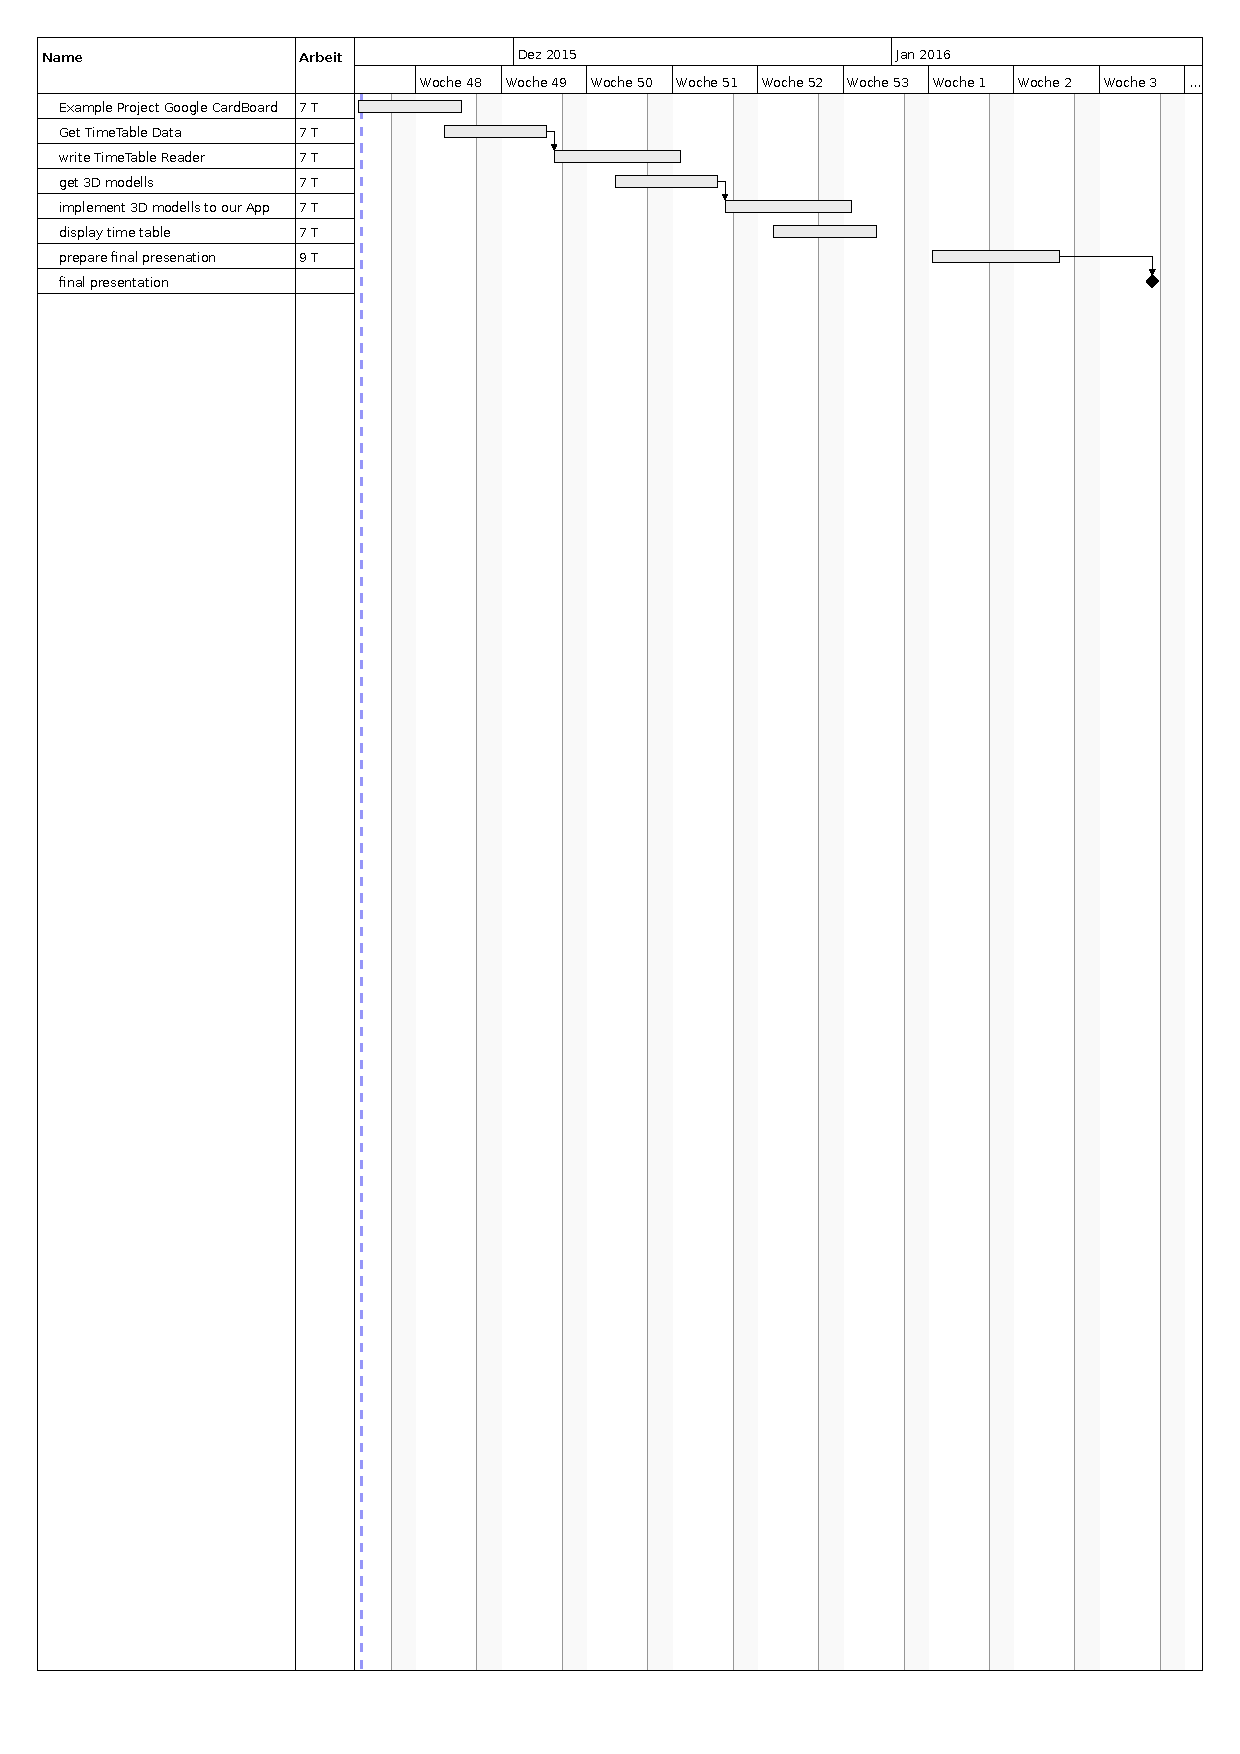
\includegraphics[scale=0.5]{chart}
\caption{Time planning}
\label{fig:method}
\end{figure}
\end{document}          
